\documentclass[12pt,a4paper]{article}

\usepackage[utf8]{inputenc}
\usepackage[english]{babel}
\usepackage{amsmath}
\usepackage{amsfonts}
\usepackage{amssymb}
\usepackage{graphicx}
\usepackage{cite}
\usepackage{hyperref}
\usepackage[left=2cm,right=2cm,top=2cm,bottom=2cm]{geometry}
\usepackage{booktabs}
\usepackage{xcolor,colortbl}
\usepackage{pstricks}
\usepackage{eurosym} 
\usepackage{longtable}
\usepackage{blindtext}
\usepackage{fancyhdr}
\usepackage{lastpage}
\usepackage{pdfpages}
\usepackage{tabularx} 
\usepackage{transparent}
\usepackage{array}
\usepackage{etoolbox}
\usepackage{float}
\usepackage{lscape}

\title{Communication logistics}
\author{Communications department}

\begin{document}
\maketitle
\section{Aim of the document}
\paragraph{}
In this documnt it will be described how the information travels since the client  asks for information of its satellite until it recives the information. This proces will be divided in 3 segments:

\begin{itemize}

\item \textbf{Grouns Segment:} is the logistics from the client to the corresponding Ground Station and vice versa.

\item \textbf{Sky Segment:} is the logistics through the constelation for comunicating with the client's satellite.

\end{itemize}

\section{Ground segment}
\subsection{Ground characteristics}

\paragraph{}
In order to define the logistics in the ground segment it has to be definded which nodes compose it and its characteristics.
\begin{itemize}
\item It will be at least 3 Ground Stations with the capacity to comunicate in every moment with, at least, one satellite of tthe constellation. 
\item The Ground station will be in a latitude between +80º and -80º in three separated longiudes of the globe.
\item The client could ask for and recive information every where in the planet wher he/she could conect to internet. 
\item In order to increse the capacity of the communication it will be possible to add more Ground Stations around the world.
\end{itemize}
\subsection{Ground logistics}
\paragraph{}
At first, when a client wants to contract our service he/she will have to descrive as the orbital and technical characteristics of its satellite. Then he/she has to ask for downloaging data of its satellite. This application will be sended, by internet, to the nearest to the satellite Ground Station. If we have GS in Terrassa, Beijing and Lima and the saellite its over Mexico, the application will be send to Lima GS, wherever the client is.
\paragraph{}
When the application arrives to the GS it will code it according to the communication protocol. This coded application will include where is the client's satellite and in what GS has to be downloaded the data. It will not include the path.
\paragraph{}
When the information is downloaded to the GS, it will be decodified and sended to the client. It will be also done by internet

\section{Sky segment}

\subsection{Constellation characteristics}
\paragraph{}In order to define the logistics of the communications, it is needed to take into account the different characteristics of the constellation and the satellites that are part of it.
\begin{itemize}
\item The constellation is formed by a series of polar, or near polar, orbital planes, covering the whole world.
\item Satellites in neightbouring planes move in the same direction (from north to south, or from south to north), creating two hemispheres. In one, satellites move from the south towards the north, and in the other satellites move from the north towards the south.
\item Each satellite can communicate with a potential client upwards, with a ground station downwards, with the next and the previous satellites in the same orbital plane, and with a satellite in eachneightbouring plane. If the adjacent plane moves in the opposite direction, the satellites will not communicate between them.
\item Each communication link is independent, therefore, a satellite can communicate across the orbital plane while at the same time is communicating across planes.
\item Moreover, each communication link has different channels to communicate, resulting in different communications happening in the same direction at the same time.
\item The constellation can be used to communicate two nodes, which can be either satellites or ground stations.
\end{itemize}

\begin{figure}[H]
\centering
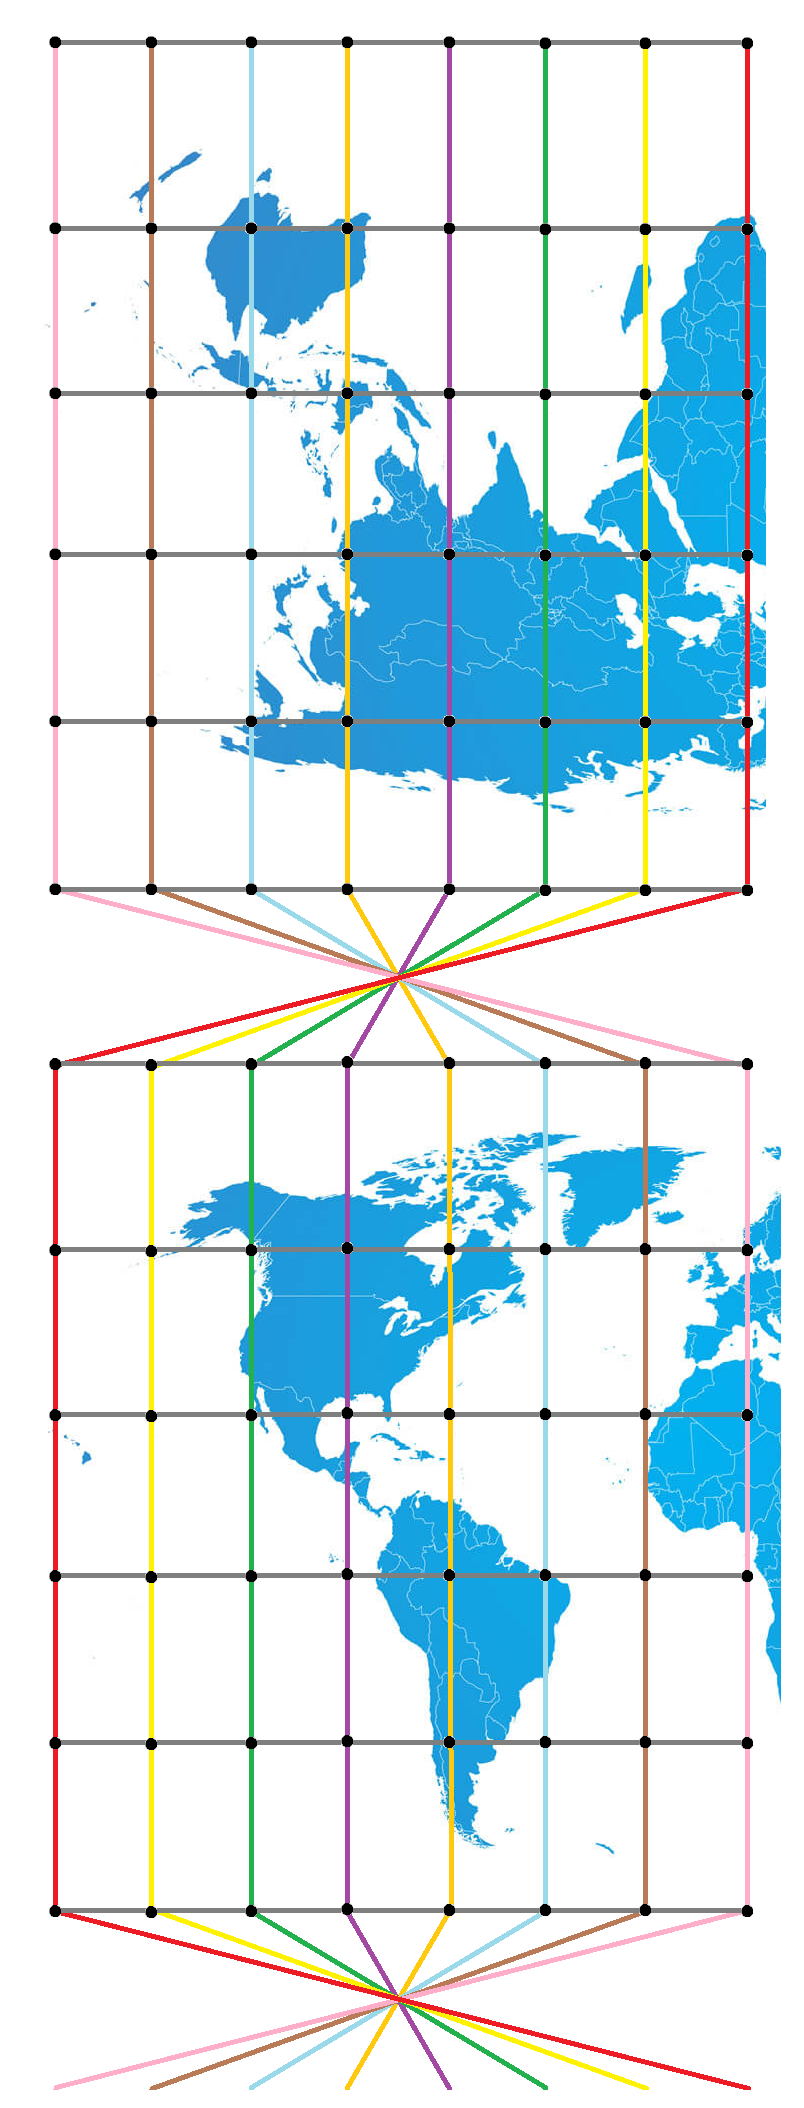
\includegraphics[scale=0.3]{network.png}
\caption[Shceme of the constellation]{Scheme of the constellation. Black dots are satellites. Color lines are communication links in the same orbital plane. Grey lines are links between orbital planes.}
\label{Scheme of the constellation}
\end{figure}
\subsection{Constellation logistics}
\paragraph{}In order to communicate properly within the network, the data to deliver will have a introductory sequence indicating its origin and its destination.\textit{Each satellite will have a map of the constellation, with the variation of the positions of each satellite and ground station over time.} Before transmitting the data, a satellite will emit a signal to the following satellite to check its status and to indicate the intention of using any of the satellite links. If the satellite is active and it is avaiable for communications, it will return a signal to indicate the avaiability. 

\paragraph{}The path that will follow the data will be the following: in the network map, the data will first travel along the orbit upon reaching the closest satellite at the destination latitude, then, it will change orbital planes upon reaching the closest satellite to the destination.

\paragraph{}In case a satellite is inactive, it can not return a signal, and the emitting satellite will not transmit to that satellite and will find and alternative route. If the satellite is active, but the intended route for the emitting satellite is alredy being used in all of the channels, it will return a signal saying that is occupied.

\paragraph{}When a satellite cannot transmit in the regular path, it will use the alternate path. The alternative path consists in first transmitting in the different orbital planes upon reaching the satellite closest to the target longitude, and then trveling along the orbital plane upon reaching the closest satellite to the target. If the alternate path is also unable of being used, the satellite will try to use the regular path once again, and will alternate with the two paths until one of them is able. Meanwhile, the satellite will store the data.

\paragraph{}From all the channels in each link, one of them will be reserved. This is the channel that will be used for the company's ground station to check the status of the constellation and giving orders to the satellites of the constellation.






\end{document}